%methods chapter
% Enough for an expert to reproduce without needing extensive references
% all data should be in thesis so they can be checked (appendix maybe and supplements)
% Methods commonly used throughout maybe leaving chapter specific methods to that chapter
\graphicspath{{chapters/2.Methods/figures}}

\chapter{Methods}

\section{Microbiology}
\subsection{Strain information}
During this project 3 \textit{Paramecium bursaria} cultures have been used.  These have been obtained from 
the UK Culture Collection of Algae and Protozoa (CCAP) and the Japanese National BioResource Project (NBRP).
Specifically:
\begin{itemize}
    \item CCAP 1660/12: European \textit{Paramecium bursaria} SW1 with \textit{Micractinium reisseri} SW1-ZK \citep{Hoshina2010}
    \item CCAP 1660/13: European \textit{Paramecium bursaria} (unknown strain) with \textit{Coccomyxa} CCAP 216/24 \footnote{This is a mixed culture 
            containing both CCAP 1660/12 strain with \textit{Micractinium} and the \textit{Coccomyxa} bearing strain, 
        the \textit{Coccomyxa} endosymbiont has been further isolated in CCAP under the description CCAP 216/24 (pers. comm. Undine Achilles-Day CCAP)}
    \item NBRP Yad1g1N: Japanese \textit{Paramecium bursaria} Yad1w with \textit{Chlorella variabilis} 1N \footnote{
        Yad1g1N host is mating type 1 and was created by mixing of isolated and 
        cultured endosymbiont (\textit{Chlorella variabilis} Clone 1 (known as 1N strain)
        }
\end{itemize}

Both CCAP cultures (1660/12 and 1660/13) were isolated from the same pond in Cambridge, UK (pers. comm. Undine Achilles-Day CCAP)
CCAP 1660/12 was the principal culture and all genomic, transcriptomic and metabolomics analyses were conducted using these cultures. 
Theoretically, these 3 cultures provide us with \textit{Paramecium bursaria} strains harbouring members of each of the 3 species of 
green algal \textit{Paramecium} endosymbiont (see \ref{chap1} for more details).

\subsection{Media and Culture conditions}
All \textit{P. bursaria} and green algae cultures are maintained in 
New Cereal Leaf-Prescott Liquid (NCL) media 
(4.3g/l \(CaCl_{2}.2H$_{2}O\), 1.6g/l KCl, 5.1g/l \(K_{2}HPO_{4}\), 2.8g/l \(MgSO_{4}.7H_{2}O\), 
1g/l wheat bran, gravity filtered via GF/C paper and autoclaved) \citep{NCLCCAP} and stored in 
a 12:12 light:dark cycle incubator at 15\celsius. 
%2x21 watt 865 daylight tubes at 2000 lumen each
Cultures were sub-cultured every 2 weeks with fresh NCL media and were inspected using light microscopy to monitor health.  
No bacteria was provided in cultures using for transcriptomics or genomics but otherwise the medium was bacterised with
\textit{Klebsiella pneumoniae} SMC (strain donated by the Meyer Lab, Ecole Normale Supérieure, Paris) the day before use. 


\section{Omics}
``-omic'' technologies are those aimed at globally characterising a class of biomolecules 
within a specific biological sample (charactising the ``-ome''). The most prevalent and developed 
are genomics, transcriptomics, metabolomics and proteomics. 
Genomics aims to detect and analyse DNA, seeking to describe and discover genes and non-coding DNA
features often for comparative and evolutionary purposes. Similarly, transcriptomics is orientated 
around the characterisation of RNA in a sample and thus to investigate RNA transcription. This can include
mRNA as well as small and non-coding RNAs and usually seeks to catalogue transcripts,
aid annotation of genomic data, investigate splicing and transcript modifications
and/or assess transcriptional response to a given condition or cellular state \citep{Wang2009}.
Metabolomics seeks to identify and quantify small biomolecules that make up the terminal and
intermediate products of cellular metabolism e.g. carbohydrates, alcohols, and animo acids.
Proteomics, on the other hand, is orientated towards the characterisation  
of proteins present in a sample. 
There are also a plethora of additional approaches which seek to characterise
different subsets of these biomolecules e.g. epigenomics (epigenetic modification to DNA such as methylation
and histone binding), gylcomics (characterisation of saccharides) and microbiomics (community genomics of organisms associated with a metazoan organism e.g. microbes present in the human digestive tract).
``Meta-\ldots-omics'' is the application of specific ``omic'' method to a biological sample 
containing multiple organisms. For example, ``metagenomics'' has been used to investigate
the cellular community composition of marine micro-eukaryotes \citep{}<++> (BIOMARKS PAPER WHEN PUBLISHED) %BIOMARKS PAPER WHEN PUBLISHED


The major benefit of ``-omic'' approaches is that of obtaining global (or near global) characterisation
without as much \textit{a priori} knowledge of the system being studied (i.e. organism,
environment etc) and much higher throughput (at a lower cost) than more targeted
approaches. For example, estimating the abundance of all transcripts using RT-PCR
would require sequence knowledge to design primers as well as an infeasible amount of
reactions to acquire a characterisation remotely similar to that obtainable by transcriptomics (RNA-Seq).
This ``non-targeted'' (or rather less targeted) approach also removes a degree of scientist-induced bias 
by omitting conscious selection of molecule specific probes.

Even so, the ability to use ``omic'' methods to investigate non-model
organisms is a relatively novel technological and methodological development.
This is due to the necessary maturation of technology and databases to provide
enough annotated resources to identify and determine the likely function of characterised
molecules. While, \textit{Paramecium bursaria} and green algae such as \textit{Micractinium
reisseri} could be considered ``model'' organisms throughout the early days of 
molecular biology that claim is weaker in terms of the genomics era
of biology (2000-today).  Particularly, when compared to such powerhouses of modern 
biology as \textit{Arabidopsis thaliana}, \textit{Mus musculus}, \textit{Saccharomyces
cerevisiae} and even ourselves (\textit{Homo sapiens}) resources to guide ``omic''
analyses of this system are relatively scant.
This potential for functional and adaptive analysis of non-model organisms using 
combined ``omics'' (i.e. genomics and transcriptomic) approaches (e.g. \citep{Munoz-Merida2013,Feldmesser2014})
has recently been demonstrated. Furthermore, it is increasingly feasible to dispense
with genomics as a pre-cursor step and conduct functional analyses using transcriptomic datasets alone.
This has been achieved even in the PbMr system \citep{Kodama2014}.

However, care must be taken with ``omics'' approaches as they can easily become purely descriptive,
not provide explanatory or mechanistic insight, not generate testable hypotheses and/or produce
models without biological relevance \citep{Fang2011}. This is generally true
for systems-level approaches, and has been raised as a concern \citep{Dougherty2008}.  
However, alternatively the methodological reductionist approaches
\footnote{
    Epistemological reductionism: ``explain all biology in terms of physics and chemistry'' \citep{Crick1966}
    i.e. biology is applied chemistry which is applied physics which is applied maths. 
    Ontological reductionism: a biological system is only the sum total of its component molecules and their
    interactions.
    Methodological reductionism: examination of simple components can be used to understand complex system \citep{Fang2011}}.
that modern biology is founded upon are not without their limitations.
On top of the lacking the benefits of ``omics'' mentioned above, by only considering elements of a system in isolation
one can omit the existence of more complex systemic mechanisms/features (or at the extreme ``emergent propoerties'') \citep{Fang2011}.  

In reality, this is a false dichotomy, both approaches are best utilised in
a complementary manner in which a systems approach is used to generate novel and interesting
hypotheses which can then be tested in isolation using reductionist methods \citep{Casadevall2008}.  
For example, generating a model of interorganism metabolism and then testing
hypotheses in this model e.g. testing that a particular protein transporter is responsible
for the transfer of metabolites that supports a particular relationship by knocking out
that transporter and observing the resultant phenotype: is the relationship perturbed predictably?



% remove if we don't use this - metabolomics vs proteomics MS MALDI-TOF
% \subsection{Mass spectrometry}
% \subsubsection{Metabolomics}


\subsection{Genomics and Transcriptomics}

They key technology behind state of the art genomics and transcriptomics is that of
DNA sequencing (whether the source template is genomic DNA (gDNA) or RNA reverse transcribed into cDNA)
\footnote{Typically, RNA molecules are characterised following
    conversion to cDNA using reverse transcriptases (RT).  There are disadvantages of this RT step, for example 
it is potentially artefact generating and error prone, and thus can complicate detection of lowly expressed
transcripts and strand-specific information. Additionally, it can place restrictions on the possible
input RNA quantity and quality. It is possible to directly sequence RNA \citep{Ozsolak2009}.
Fortunately, this method shares most of its basic mechanisms with DNA sequencing, specifically 3rd generation single molecule 
sequencing \citep{Ozsolak2011} but has only been commercially available with the now defunct Helicoscope.}
These technologies can largely be divided into 3 technological eras with today (2015) 
broadly at the transition between 2nd and 3rd generations.

1st generation sequencing technology originates in 1970s with the work of Sanger \&
Coulson \citep{Sanger1975,Sanger1977,Sanger1977a} which 
developed the principal of chain termination during synthesis and subsequent relative fragment size determination. 
Briefly, by having 4 separate reactions in which PCR terminates on the incorporation
of dideoxy nucleotides (ddNTP) corresponding to each of the 4 principal DNA bases (i.e. ddATP, ddGTP etc.) 
you can generate a series of DNA fragments of various sizes.  Size fraction separation of these fragments 
using gel electrophoresis means the DNA sequence can be easily read from the fragment size distribution
across the 4 ddNTP reactions \citep{Sanger1977a}. This
technique was used to sequence the first DNA genome (bacteriophage \(\phi X174\) \citep{Sanger1977}).
The metholodogy was subsequently improved by use of flourescently labelled ddNTPs by Leroy Hood,
massively simplifying automation of the process \citep{Smith1985,Smith1986}.
Further improvements followed throughout the 1990s and early 2000s with dye-termination, capillary electrophoresis
and general throughput and length automation. 
One of the most successful commercial sanger sequencing platforms is that of
highly automated 96-reaction Applied Biosystem's 3730XL capillary sequencer \citep{Bonetta2006}.
While, surpassed in throughput by later techniques, Sanger sequencing remains the gold standard for 
cheap, rapid, high quality 300-1000bp sequencing and has extensive use for targeted approaches such as 
cloning confirmation \citep{Bonetta2006,Tsiatis2010}.  
Transcriptomic analysis without prior genomic sequence data 
was possible using Sanger sequencing in the form of EST or cDNA sequencing \citep{Adams1991,Gerhard2004}.
In which partial or complete cDNA was generated from transcripts, cloned and sequenced.
Although these approaches did allow transcriptomic goals such as resolution of different isoforms without pre-existing genomic information
and aided annotation \citep{Adams1991}. Accurate relative expression levels were not resolvable beyond broad inferences
on expression enrichment of highly expressed transcripts from the proportion of the cDNA/EST library they made up.

Additionally, scaling 1st generation methods to whole eukaryotic genomes or transcriptomes 
rapidly became infeasible for most research. The scale of the human genome project \citep{Lander2001,Venter2001} is testament to that 
(20 public centers in 6 countries 
\citep{Collins2003} and \($70m\) \citep{Pettersson2009}).  


2nd generation sequencing emerged commercially in 2005 with the work
of both George Church and 454 Life Sciences \citep{Margulies2005} and featured
reduced individual reaction volumes and thus greater parallelisation (and so throughput),
cell-free preparation not requiring time-consuming cloning of DNA fragments into bacterial vectors to generate
clonal templates for sequencing, and direct sequencing detection obviating the need
for electrophoresis \citep{Jaszczyszyn2014}.
%which reduced necessary volume for 
%step-wise ``pyrosequencing'' \citep{Ronaghi1996} reations possible \citep{Schuster2008}. 
These technologies generate huge amounts (on the order of \(10^{6}-10^{9}\) relatively short (on the order of \(10^{1}-10^{3}\)bp) DNA sequences 
    (reads) randomly sampled from the input (c)DNA.  
Available 2nd generation platforms include 454's GSLFLX and GSJunior (now Roche),
Ion Torrent's (now Life Technologies) PGM, Applied Biosystem's (now Life Technologies) SOLiD and Illumina's (formerly Solexa) 
HiSeq, MiSeq and NextSeq \citep{Nederbragt2013}.

\begin{figure}
    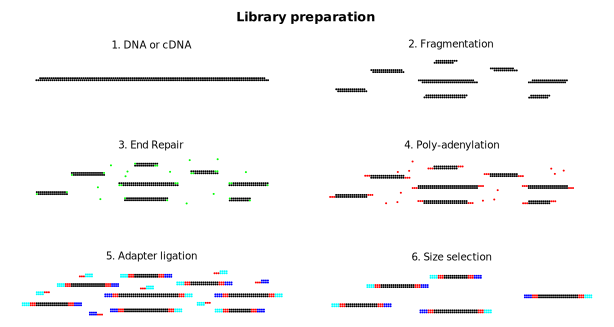
\includegraphics[width=\textwidth]{illumina_lib_prep.pdf}
    \label{fig:libprep}
    \caption{A brief overview of library preparation for Illumina}
\end{figure}


Although these platforms use a range of different implementations and largely exhibit trade-offs between read number and read length they all largely follow the same basic process \citep{Shendure2008}:
\begin{enumerate}
        \item Library generation: Randomly fragmenting input DNA into short fragments of a specific size
            followed by ligation of adapter sequences with some platforms allowing development of ``paired-end'' or ``mate-pair'' libraries in which
            each end of a fragment is sequenced separated with a known size unsequenced fragment aiding subsequent assembly.
        \item Clonal amplification: Generation of clonally identical spatially distinct clusters of DNA mainly via emulsion PCR \citep{Dressman2003} (SOLiD, Ion Torrent, 454)
            or bridge PCR \citep{Adessi2000,Fedurco2006} (Illumina) 
        \item Sequencing-by-synthesis: In which a complementary DNA strand is generated base by base via sequentially flooding and clearing a
            chamber with each dNTP and a polymerase (or ligase in the case of SOLiD).  On incorporation of a base into a cluster a detectable signal is released such as emission of certain wavelengths of light 
detectable using optics (e.g. Illumina, 454, SOLiD) or release of hydrogen ion (e.g. Ion Torrent).
\end{enumerate}

The currently dominant 2nd generation technology is that of less cumbersome \citep{Shendure2008} Illumina's bridge amplification
paradigm - specifically the HiSeq, NextSeq, and MiSeq platforms.  
The HiSeq2500 is by far the highest throughput individual platform (not counting the multi-machine HiSeqX's) able to generate up to 
400M 125bp reads per run (1TBase of data) \citep{Nederbragt2013}.
Illumina's platforms are estimated to generate 90\% of all sequenced DNA data as of 2014 \citep{Regalado2014}.

\begin{figure}
    \includegraphics[width=\textwidth]{illumina_PE_seq.pdf}
    \label{fig:libprep}
    \caption{A brief overview of paired end sequencing in an Illumina flowcell after library preparation, derived
        from \citep{Mardis2008} and Illumina 
\end{figure}


Not only has this explosion in sequencing throughput driven a massive decrease in per-base sequencing cost
leading to a subsequent explosion in available data it has also allowed the development of 
RNA-Seq (high throughput sequencing of cDNA generated from cellular RNAs).

One other innovation required for effective RNA-Seq is means of enriching fractions of RNA.
Owing to the overwhelming amount of ribosomal RNA present in a cell (or selection of cells) to avoid
wasting many sequencing reads on these instead of the mRNA or ncRNA of interesting it is necessary
to enrich extracted RNA samples.  For eukaryotic mRNA enrichment this can be easily achieved by
using poly-T primers during RT which selectively bind to the poly-adenylated tail of these messenger 
transcripts.  However, for bacterial/archael work and transcriptomic analyses focussing on non-poly-adenylated
trascripts such as ncRNAs/siRNAs/miRNAs etc. ribosomal depletion is used.  This is a process by which 
ribosomal probes are attached to magnetic beads. Ribosomal RNAs bind to these probes and the magnetic
beads can be used to partition the majority of ribosomal sequences away from the other RNA.
While, 2nd generation sequencing has driven down per-base sequencing costs the cost of library preparation 
has fallen more slowly \citep{Blainey2013}.
For this reason, combined with the higher throughput it has become common to multiplex difference samples 
during sequencing runs.  Multiple distinct samples can be be sequenced
in the same reaction (e.g. flowcell lane for Illumina platforms) by adding an indexed tags during library
preparation.  These tags can then be used to partition the reads back to their original separate samples
after sequencing. 


Finally, 3rd generation technologies are generally known as single-molecule sequencing.
These platforms still use the sequencing-by-synthesis concept but omit the generation of
clonal clusters (by emulsion or bridge PCR) by using highly sensitive detection methods to
determine base incorporation in indvidual strands of DNA.
The benefits of these approaches are that they allow avoiding the bias and error prone 
amplification step present in 2nd generation sequencing.  They also allow 

are avoiding the bias and error prone elements of the DNA sample 
preparation process allowing smaller amounts of input DNA as well as potentially degraded samples.
RNA can also be directly sequenced without the reverse transcription step to cDNA \citep{Ozsolak2009}.
Additionally, in the case of the MinIon and PacBio longer reads can be generated even than Sanger
sequencing methods (1kb to 1mb) 

The first 3rd generation platform was that of the now defunct Helicos Bioscience's Helicoscope \citep{Harris2008}
based on breakthroughs in the resolution of fluoresence visualiation using paired FRET methods \citep{Braslavsky2003}.
However, currently the main mature platform is that of Pacific Biosciences PacBio RS.  The PacBio
operates by using nanostructures known as zero-point waveguides with DNA polyermases fixed
at the bootom of to increase resolution for detecting
fluorescent signals for incorporation of bases while reducing incidental noise ``leaking'' between 
cells.  The platform-specific disadvantage of the PacBio RS is the price and size of the platform.

The MinIon differs in that is doesn't do sequencing-by-synthesis, but rather feeds DNA strands incrementally
through a biological pore protein and detects the identity of the protein using the biophysical profile.

Unfortunately, partly as an element of their recent nascence and partly due to the
poorer signal:noise of single molecule approaches instead of analysing large 
batches of identical DNA sequences 3rd generation technologies have a relatively high error rate.
Thus, currently at least, are inadequate for most eukaryotic assembly tasks by themselves.
Where they have shown great utility is in conjunction with 2nd generation datasets
as a scaffolding tool i.e. producing long noisy reads upon which more accurate but shorter
reads can be assembled.

PacBio generates 20kb and longer reads but has a high cost and high error rate (14\%) \citep{Jaszczyszyn2014}


It should be noted that there are other approaches to DNA sequencing (and characterisation of 
transcriptomes) specifically that of hybridisation based methods.  The most famous of these,
and indeed the principal way by which transcriptomics was conducted prior to the maturity of
RNA-Seq via DNA sequencing platforms is that of microarrays largely popularised by the Agilent
arrays.  These involve the binding of
fragments of complementary DNA to a tiled array with a fluorescent marker.  This fluorescence
can be detected and either relative expression level of the corresponding transcript evaluted
or in the case of genomics, the presence of a particular sequence variant determined.  
Microarrays suffer from requiring more prior information to effectively generate that direct
sequencing methods, they also lack the ease of analysis due to the continuous nature of their output
and extensive processing is required to convert relative fluorescence values at points into biologically
relaevant and comparable scales.  However, they do have the advantage of very high throughput and quick
analysis with established arrays and thus are best suited for approaches such as medical diagnostics
and detection of SNPs in well characterised genomes such as the human genome.

Microarrays also required pre-existing genomic sequence to design arrays, had limited sequence resolution,
were difficult to use to distinguish alternative isoforms or allelic expression, as well as having relatively
poor dynamic range in recognising different transcription levels.  While microarrays are higher throughput
than older EST sequencing even that allowed isoform distinguishing but did lack accurate evaluation of 
gene expression. \citep{Wang2009}




Therefore, all genomic and transcriptomic sequencing in this PhD has been performed using the 2nd generation
Illumina HiSeq platform due to its relative maturity, high-throughput, relatively accurate
paired-end output making it currently the most amenable platform to effectively
use \textit{de novo} genomic and transcriptomics approaches.  Additionally, Sanger sequencing
has been used when accurate targeted sequencing was called for, such as investigating the
taxonomic distribution of \textit{Paramecium} green algal endosymbionts (see \ref{chap1}).



\subsubsection{Single Cell Sequencing}


While the quality of the output of earlier sequencing techniques
was highly reliant on both the quantity and quality of the input DNA (or cDNA) (not to mention
characterisics such as GC\%) precluding many systems from easy analysis.  This is especially
problematic for the majority of systems that are not easily culturable and thus can't be
grown up in sufficient quantities to easily extract sufficient nucleic acids to conduct.



Starting with single-cell single-gene sequencing experiments (e.g. \citep{Kuppers1993}) 


Single cell sequencing allows obtaining data directly from individual cells
avoiding the bias and complication of culturing or have to decompose a complex environmental
metagenome or metatranscriptome containing a plethora of diverse cells \citep{Blainey2013}.  It also allows 
investigation of cells at particular life stages e.g. sexual reproduction without difficult
and potentially biasing synchronisation methodologies.  



Currently, single cell genomics still requires whole genome amplification (WGA) even with 
3rd generation sequencing platforms due to the relatively inefficient library preparation
methods requiring relatively more starting material than is avaiable in the DNA extracted
from a single cell (on the range of nanograms). \citep{Blainey2013} %%find support quote for transcriptomics needing WGA too




Single cell methods use multiple-displacement amplification to increase the concentraion of
nucleic acids 

For example. the Qiagen Repli-G kit used for both single cell transcriptomic and genomic analysis
of the \textit{PbMr} system.

Transcripts are reverse transcribed and then ligated into larger fragments.  MDA
is then undergone on the larger fragments before the usual library preparation process.

MORE DETAILS ABOUT THE METHOD


One interesting consideration for single cell transcriptomics is the possible generation
of chimeric reads that will cross the boundary between two randomly ligated transcripts.

However, the risk of this can largely be mitigated by selection of a relatively small fragment
size for paired end sequencing.

5'-3' - 5'-3'  - sequencing primers are unlikely to rpim



\subsubsection{Assembly}

All major 2nd and 3rd generation sequencing platforms output a FastQ formatted file.
These are files containing the sequence of a read and a per-base quality score known as a Q score.
These scores (Q) are calculated as a logarithmic relation to the base-called error probability (P)
\[ Q = -10\log{10}{P} \]
and conversely: 
\[ P = 10^{frac{-Q}{10}} \]
Therefore \[Q = 30 \] corresponds to 99.9\% base call accuracy


\textit{De novo} transcriptome and genome assembly 



\begin{figure}
    Summary of stages of illumina sequencing
\end{figure}



\textit{de novo} assembly


Spades \citep{Bankevich2012}

Trinity \citep{Grabherr2011}


\subsection{Assessing Assemblies}

RSEM-eval, mappings, NG50, L50, N50

Assemblathon 1 \citep{Earl2011}
GAGE \citep{Schatz2012}
Assemblathon 2 \citep{Bradnam2013}
Nucleotid.es: Linux Container (specifically Docker \citep{Merkel2014})  based continuous assembly evaluation using QUAST \citep{Gurevich2013a})


\subsubsection{The Problem with Ploidy}

One important complication in the assembly on eukaryotic genomes 
relative to bacteria or archael sources is the issue of highly heterozygous polyploid genomes.
This is problematic as the de Bruijn graphs constructed during assembly
rapidly increase in complexity when reads from heterozygous samples become
incorporated \citep{Kajitani2014}.  This is because k-mers derived from heterozygous regions of 
homologous chromosomes will partition the assembly graph into bubbles that cannot be easily 
or accurately resolved by most assemblers expecting only limited structural variation during
assembly.  Previously, attempts to work around this included inbreeding to generate
homozygous lines or fosmid based approaches.

Specialised genome assemblers have been produced to address this problem,
for example Platanus performed well on both highly and lowly heterozygous 
genomes using k-mer autoextension approaches and by merging haplotypes
at both contig assembly and scaffolding steps, as well as incorporation
of various heuristics involving bubble resolution \citep{Bradnam2013,Katjitani2014}

Likewise, transcriptome assembly complexity rapidly increases with the number of alleles
expected per gene determined by ploidy, heterozygosity and complex gene families
and in turn how many transcripts per allele in light of alternative splicing.

This is particularly problematic in the PbMr system owing to the massive
ploidy of the host \textit{Paramecium bursaria} and the numerous whole genome
duplications in its relatively recent evolutionary history (1).  This also 
explains the difficulties in using sister species, as the most sequenced Paramecium
genus species are the aurelia complex which have undergone 2 WGD since divergence with
\textit{P. bursaria} \citep{McGrath2014}.



\subsubsection{Genomics}
%Project standards:
%Standard Draft: Minimally filtered, incomplete, assembled into contigs, may have poor regions and be incomplete, may have some contamination
%High-quality Draft: coverage of at least 90\% of genomes or target regions, contamination exluded, little manual review, still might be seq errors or misassemblies, no implied order and oreintation to contigs (can be assessed for gene content)
%Improved-high quality draft: manual or automated additional work, gap resolution, no obvious missassemblies, normally adequate for comparison with other genomes
%Annotated-Directed Imrpovement: Overlapping, improved with annotation, verified, gene models etc useful for gene comarpsiosns, alt splicing, pathway reconstruction
%Noncontiguous finished: high quality, finished apart from a few repeats or gaps, good enough for almost all analayses
%Finished: gold standard, less than 1 error per 100,000, replicon in contig seqs, reference quality \citep{Chain2009}




\subsubsection{Annotation}

Reed \textit{et al.} \citep{Reed2006} divided components annotation into a useful dimension paradigm as follows:
\begin{enumerate}
    \item Enumeration: identification of genes and assignment of their predicted or known functions. What?
    \item Interaction: integration of protein-protein, regulatory and metabolic interaction data between components Can they interact?
    \item Genomic Localisation: analysis of genomic localisation of genes i.e. epigenetics.
    \item Plasticity: investigation of the change of other dimensions over evolutionary time. Does their interaction change over time? \citep{Reed2006} 
\end{enumerate}

Clearly, at a systems level it is difficult (if not impossible currently), 
even in well defined model organisms, to complete a full 4-dimensional annotation 
for all cellular components. However, it is more than feasible to have a largely
complete 1D and even 2D annotation with 3D and 4D investigated for specific 
components.  Furthermore, annotation can be conducted with a range of confidences
from in silico predicted interactions to biochemically validating those predictions in vivo
and incorporating the precision and recall of various methodologies. Generally, such a process
is inherently iterative with successive model building and experimental testing and validation 
or rejection of such models \citep{Reed2006}.

One of the major goals of this thesis is to reconstruct a preliminary predicted
2D annotation of the PbMr system.

The most important step towards this goal is that of eukaryotic gene prediction.


Eukaryotic gene prediction is achieved by generally two methods - \textit{de Novo} HMM based
methodologies (e.g. GENESCAN, TWINSCAN \citep{}<++>) and expression evidence based methods
in which reads from sequenced cDNA (or in older approaches ESTs) are aligned to the 
assembled genomic contigs \citep{Brent2007}.  Unfortunately even relatively deep
sequencing of cDNA can fail to identify the structure of 20-40\% of genes in a typical
eukaryote genome owing to these genes being expressed only at very low levels or in
different conditions than that from which the cDNA was extracted \citep{Brent2007}.






\subsection{Transcriptomics}


While generally computationally simpler than genomic assembly \citep{MacManes2014}
owing to the relatively fragmented nature of transcripts compared to genomic 
sequences (i.e. lots of transcripts of various lengths rather than several 
long chromosomes).  There a few key challenges to transcriptomic assembly
that is absent in genomic work specifically:
\begin{itemize}
    \item Handling assembly of alternative isoforms of transcripts \citep{Pyrkosz2013}
    \item Assembly of transcripts from gene-dense genomes with overlapping 5' UTR 
    \item Assembly of data with highly heterogeneous read coverage, as transcript
        expression level is proportional to read coverage (indeed expression analysis
        using RNA-Seq datasets relies upon this fact).
    \item Random hexamer bias
    \item GC content bias, particularly so in PbMr
\end{itemize}

These problems are particularly problematic in \textit{de novo} approaches,
however referenced assembly has its own issues in transcriptomics






The correlation of transcript level to protein level is difficult





Unfortunately, conventional RNA-seq requires either an established moderate-to-high
density culture of the organism of interest 








http://rnaseq.uoregon.edu/
http://bioinformatics.bc.edu/marthlab/scotty/scotty.php

Experiemntal design, read depth, ENCODE, Tarazona S 2012 fdiff exp in RNA-seq
a matter of depth

\begin{itemize}
    \item Check Quality (FASTQC)
    \item Trim reads (Trimmomatic)
    \item Re-check quality (FASTQC)
    \item Error-correct reads (?)
    \item Normalize coverage (khmer)
    \item Test paramters for multiple assemblers
    \item Run each assembler with best parameters
    \item Analyse all and merge best assemblies
    \item Annotate transcriptome
    \item Map reads to assembly, count
    \item Differential expression analysis
\end{itemize}










Further complications from single cell:
Fusions are created in cDNA ligation step prior to MDA in WTA
However, poly-A tails should mean fusion reads are unlikely as they need to a
span poly-A trac in all 4 possible fusions apart from 3'-5':5'-3'
So to get high levels of chimeric reads we would need the two same transcripts
in the same fused orientation multiple times.  Otherwise any other 3'-5':5'-3'
fusions should be fairly rare so likely discarded in error-correction etc steps

\subsubsection{Quality Checking}

FastQC tool and its parameters

\subsubsection{Read trimming}

% /storage/fin/raw_reads/raw_sct_reads/optimising_trimming_paramters/test_mapping_to_bulk


Currently, there is no clear answer to the question, which is the best trimming algorithm.
This is due to many dataset-specific effects as well parameter-dependence \citep{DelFabbro2013}.
However, 



Trimming algorithms can be divided into two groups: running-sum based approaches e.g. Cutadapt and ERNE-FILTER
and window-based e.g. FASTX, PRINSEQ, Sickle and Trimmomatic \citep{DelFabbro2013}.












Difficulties: 
A major source of bias in transcriptomic datasets is that of compositional biases induced
by the random hexamer priming used in the generation of cDNA in many library preparations.
(see \ref{}<++>) %previous section of sequencing itself %does SCT kit do random hexamers?
Specifically, these random hexamers do not bind uniformly across the transcripts,
therefore the location of reads are not uniform \citep{Hansen2010}\citep{Hansen2010}.
Fortunately, the single cell kits do not utilise random hexamer priming {}<++> %Check with DAVID
So despite inducing other biases, they do not induce this one!


Another source of bias is the strong correlation between GC richness in read coverage
observed in 2nd-generation Illumina sequencing \citep{Dohm2008,}
This is possibly to do with the different biophysical properties of GC-rich dsDNA (high melting point) \citep{Dohm2008} %is this relevant?
Or biases in PCR -ampligication, or specifically i9n bridge PCR of cluster amplification


Errors are more common at the start and end of 




Sequencing errors: Illumina sequencing has non-random error distribution across length of read, increasing towards the 3' end liu2012. These errors are generally substitution errors yang2013 at a rate of 1-3\% globally \citep{MacManes2014}.  However, while the latest assemblers (see \ref{}<++>) are capable of %ref to assembly section
handling many of these errors, inevitably sequencing error does cause some
assembly error MacManesANDEISEN2013.
Furthermore, errors rapidly increase both the space and time complexity of the assembly (discussed in \ref{}<++>) problem \citep{MacManes2014}.

One of the most important and prevalent methods to try and improve assembly
accuracy in the face of sequencing errors is that of read trimming, typically
using one of a range of tools: TRIMMOMATIC, SICKLE, FASTX-TOOLKIT, BIOPIECES \citep{}<++>. %citations for tools

Trimmomatic is the preferred tool of choice as it more read-pair aware than
FASTX-TOOLKIT and BIOPIECES, retaining pair ordering and conducting more
advanced trimming checks using pairing information such as adaptor read-through.
By retaining pairing information and outputting ``surviving'' paired reads and
unpaired reads TRIMMOMATIC precludes lengthy repairing of header pairing information
in large datasets. \citep{}<++> %More information about how trimmomatic oworks and comparison to other trimmers

The main approaches used individually or as a combination in trimming tools are that 
of adaptor trimming (identifying and removing sequencing adapter sequences from reads),
sliding windows (removing nucleotides that fall below a provided average quality threshold),
basic terminal quality trimming (remove individual 5' or 3' nucleotides that have an associated PHRED score
below a ceratin threshold) and minimum length (discard reads that fall below a minimum length). 
\citep{}<++> %citations explaining these methods

The key difficulty is that all widely used tools above require user-defined thresholds
for the various trimming parameters e.g. for sliding window approaches - a window size
and a minimum average quality threshold over the window.  
This leads to a careful trade-off, if conservative/aggresive (i.e. high) quality thresholds
are used many reads will be discarded, reducing the amount of data from which to 
construct an assembly.  This will reduce feature resolution such as alternative splices 
and in will lead to the loss/reduced assembly accuracy of lowly expressed (but potentially biologically interesting) transcripts \citep{MacManes2014}. On the otherhand, instinctually if permissive (i.e. low)
quality parameters are set then potentially erroneous reads will be incorporated into the assembly
and global assembly accuracy will decline. 

Relatively little work on the optimisation of these parameters has been conducted, and generally
researchers conducting high-profile \textit{de novo} assemblies utilise aggressive thresholds \citep{MacManes2014}.
However, for \textit{de novo} transcriptome assembly assessed using a range of metrics
(e.g. mismatches to previous datasets, kmer number, PE reads mapping back to assembly etc.)
most of the gain of assembly accuracy occurred at a threshold of \[\geq 5\].
Particularly, low abundance kmers are largely discarded with a threshold of \[\geq 5\].
Suggesting, that a very low threshold of 2 or 5 optimises assembly quality potentially
followed by kmer abundance based error correction \citep{MacManes2014}.



% TRY THIS FOR SCT








\subsubsection{Error correction}

While second-generation sequencing technologies have massively increased
throughput on an individual read basis they exhibit a much higher error
rate than earlier Sanger approaches with Illumina HiSeq reads showing \[0.5-2.5%\]
error rate \citep{Kelley2010}.  

These errors complicate assembly as they will rapidly increase
the complexity of the de-Bruijn graphs 

Typically the most widely used error-correction algorithms for 2nd-generation
sequencing reads. 


While explained later in \ref{Assembly}, generally OCC assembly is reliant on 
fast and accuarte overalp calculations while de Bruijn approaches require
robust error correction \citep{Palmer2010}.



Single-cell genomics sequencing reads display high variance in their coverage 
across the genome with some sections. Previously error correction tools (such as
QUAKE \citep{Kelley2010}

\citep{Nikolenko2013}

Sequence error correction improves \textit{de novo} assembly \citep{MacManes2013}









\subsubsection{Digital normalisation}

\subsubsection{Assembly}
Optimising parameters
Theory
Combining


Almost every \textit{de-Novo} assembly algorithm use one of two approaches:
overlap-contig-consensus (OCC) e.g. Celera etc
de Bruijn is more widely used but even as recently as 2010 it was unclear
which approach was superior \citep{Palmer2010}.
However, it has become rapidly evident with further expanding sequencing capacity





Assembly assessment:
Adapter trimmed PE reads concordantly mapping to assembly \citep{MacManes2014} 
Number of complete ORFs (start and stop codons) using TRANSDECODER 
Unique transcript number using BlastP (80\% similarity over 100aa and e-10)
Expression for each contig https://github.com/macmanes/trimming_paper/tree/recreate_ms_analyses/scripts


\subsubsection{Annotation}

\subsubsection{Mapping}

The tradeoff between read-mapping sensitivity (number aligned) and specificity (number correctly aligned)
Modern aligners overcome most errors making trimming unecessary \citep{DelFabbro2013}





However, studies on simulated datasets have shown that the main sources of error
when conducting mapping to a reference transcriptome to infer expression counts
the most important sources fo error are splice variants and missing transcripts
\citep{Pyrkosz2013}.  Interestingly, this paper also found that different mapping
strategies did not yield substantial differences in mapping quality \citep{Pyrkosz2013}.

When mapping RNA-Seq data there is diminishing returns with 1M reads providing 
approximately the same level of accuracy in estimate transcript abundance 
as >30M reads for highly-expressed gene in six standard model organisms \citep{Lei2014} 




\section{Machine Learning and Statistical Pattern Recognition}

Machine learning (ML) is a field of computer science 
devoted to the challenge of developing and applying algorithms capable of 
automatically inferring and utilising patterns in data \citep{Murphy2012}.
A formal definition of machine learning is:
``A computer is said to learn from experience E with respect to some class of tasks 
T and performance measure P, if its performance at tasks T, as measured by P, improves 
with experience E.'' \citep{Mitchell1997}
ML encompasses techniques and methods from various areas including statistics,
pattern recognition, optimisation/control engineering, neuroscience and artificial intelligence.
Applications range in complexity from simple linear regression to deep convoluted neural networks 
with millions of free parameters running on dedicated super-computers \citep{Wu2014} 
which are capable of beating human-performance on complex image classification tasks 
(e.g. IMAGENET \citep{Berg2014,He2015}).

Typically, we seek to set the parameters (\theta) of a function in such a way
that another property is minimised.  For example, in linear regression we try to find 
parameters of a straight line \(h_{theta}(x) = \theta_{0} + \theta_{1} * x_{1}\) which minimise the distance
between the line and the data (usually the sum of squares distance).
This distance/error is calculated using something known as the cost function e.g. \(J(\theta) = \frac{1}{2} \sum^{m}_{i=1} h_{\theta}(x_{i}) - y_{i})^2\) (where \(m\) is the number of \(x, y\) pairs in the dataset for linear regression.  
Most algorithms will seek to minimise the value of this cost function \(J(\theta)\) with respect to 
the parameters of the original function \(h_{theta}(x)\).  Typically, this is achieved using a variety of algorithmic optimisation techniques.
The most prevalent of these are gradient descent based methods in which the value of \theta is modified 
in the direction of the gradient of the cost function (determined using the partial derivative of \(J\) with respect to \theta: \(\frac{\partial J_{\theta}}{\partial\theta}\)).  
The choice of model is important as it determines how well this error can be mininmised for the current data.
It also determines how well this will generalise to new data.

\begin{figure}[h]
    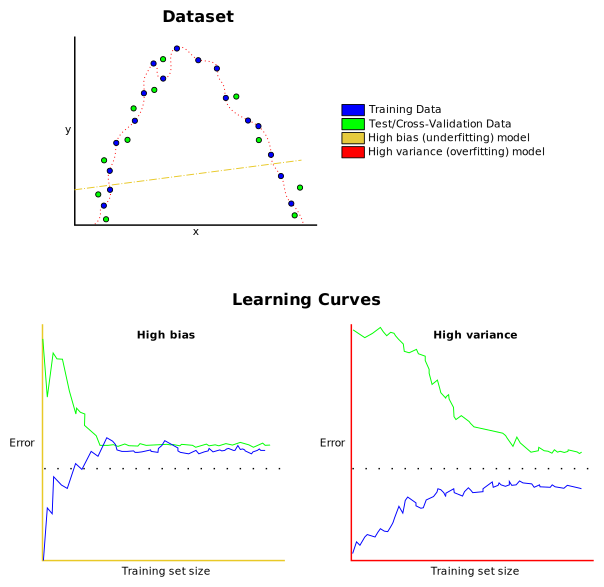
\includegraphics[width=\textwidth]{fitting.pdf}
    \caption{Plot showing a high bias (underfit) model in yellow and a high variance (overfit) model in yellow.
        Below are learning curves corresponding to each of these respectively.
        Learninv curves show the effect of different training set sizes on the training and test error of misspecified models.
        Overfitted models show a large gap between test and training errors, they fit to the training data well but don't generalise
        to new data (i.e. test data).
        Underfit models show a very high training error and little difference between test and training data as the model is too simple
        to fit the training data at all.
    }
    \label{fig:fitting}
\end{figure}


Machine learning can be split into 3 basic components: representation (the form of the model e.g. and input) in which 
evalution (cost functions) and optimisation (gradient descent) \citep{Domingos2012}

%Similar to statistics in general, approaches can be parametric or non-parametric in machine learning and can
%be easily distinguished by the change in numbers of parameters are training set size increases.
%For parametric approaches the number of parameters are fixed and finite e.g. when fitting a gaussian distribution
%to a dataset the only parameters are mean and variance of the distribution no matter how many data points are used.
%Non-parametric models on the other hand have an increasing number of parameters as the training set
%increases in size e.g. Dirichlet processes.  Typically, parametric models are faster but are less flexible as
%they make more assumptions about the dataset, whereas non-parametric approaches can be computationally infeasible
%for large datasets \citep{Bishop2006}.
%\section{Fitting}
%``Curse of dimensionality'': as the number of input/feature dimensions increase any training dataset
%will become increasingly sparse.  Parametric models are one solution to this.


Machine learning is typically divided into 2 main subsets depending on the nature of the dataset involved: 
supervised learning (e.g. classification and regression) and unsupervised learning (e.g. clustering,
density estimation and dimensionality reduction).
There are also approaches that blend features of both supervised and unsupervised learning known as semi-supervised
learning as well as an alternative idea known as reinforcement learning built on the premise of the psychology
of behaviour and the indirect reward of trial and error approaches \citep{Bishop2006}.

\subsection{Supervised Learning}

In supervised (also referred to as predictive) learning the principal aim is 
to learn a mapping between inputs/features \(x\) and outputs/response \(y\) from a set of 
inputs and their corresponding expected output.  This is known as the training set 
i.e. \(\mathcal{D} = {(x_{i}, y_{i}) \forall i \in N}\) where \(N\) is 
the cardinality of the training set \citep{Murphy2012}.  
A supervised learning algorithm thus seeks to approximate \(y=f(x)\) where \(f\) is an unknown 
function. This estimated function \(\hat{y} = \hat{f}(x)\) (see \ref{eq:sup}) would then generally
be applied to new data known as the test data for which the expected outputs are not known (i.e. 
\(x_{i} \not \in \mathcal{D}\)).

\[
    \begin{bmatrix}
        x_{0,0} & \cdots & x_{0,j}\\
        \vdots & \ddots & \vdots \\
        x_{i,0} & \cdots & x_{i,j}\\
    \end{bmatrix} \overset{\hat{f}}{\rightarrow} \begin{bmatrix}
        y_{0} \\
        \vdots \\
        y_{i} \\
    \end{bmatrix}
    \label{eq:sup}
\]

Supervised learning is further subdivided into two approaches depending on the nature of the expected
outputs: classification and regression\footnote{It is worth noting that the somewhat confusingly named
    ``logistic regression'' is typically a form of classification}.

In regression the desired outputs are real-valued (or ordinal) i.e. \(y_{i} \in \mathbb{R}\) and we seek to
estimate a particular output quantity for a specific input.
The simplest example of this would be the 2-dimensional linear regression problem mentioned above in which
we are determining the parameters of a line (gradient/weight and intercept/bias) which best fits the training 
dataset (\(\mathcal{D}\)) composed of pairs of \(x\) and \(y\) values.  Once this line has been found we 
can use it to predict the value of \(\hat{y_{i}}\) for data in the test set \(x_{i} \not \in \mathcal{D}\).


On the otherhand, in classification applications are supervised learning problem in which the expected outputs are 
categorical or nominal variables such as class labels like ``host'' and ``endosymbiont'' 
(\(y_{i} \in {host, endosymbiont, ... C}\)).  These classifications can be binary (two possible outputs i.e. 
\(y={0,1}\)), multiclass (\(\left\vert{{y}}\right\vert > 2\)),
or multi-label (similar to multiclass but outputs aren't mutually exclusive, i.e. an input can belong
to multiple classes) \citep{Murphy2012}. 


Supervised learning algorithms can additionally be either probabalistic or non-probablistic and generative or 
discriminative.
Probabilistic functions will return a probability distribution associated with possible class labels or
regression values whereas non-probablistic approaches will only return the most likely class label or value.
Continuing 
Generative algorithms, such as Naive Bayes, seek to model the process by which the output data was generated 
from the input i.e. learn the joint probability \(p(x,y)\) and make predictions on that basis via Baye's Theorem (see \ref{eq:bayes}) 

\[
    p(x,y) = p(x|y)p(x) = p(y|x)p(y)
    p(y|x) = \frac{p(x,y)}{p(y)}
    p(y|x) = \frac{p(x|y)p(y)}{p(x)}
    \label{eq:bayes}
\]

Whereas, discriminative classifiers, such as logistic regression/linear classifiers,
model the posterior probability \(p(y|x)\) directly or just learn mappings in the case of non-probabalistic approaches.
In other words, for classification problems a generative model would determine the statistical distribution of 
individual classes whereas discriminative models would just determine the boundaries between them.
Generative models often perform better on small training sets by preventing overfitting with discriminative
classifiers performing better as the training set grows \citep{Ng2002}.


%Generally, our functional approximation is probablistic - it will return the most
%probable class label \(\( \hat{f}(x) = \argmax{C} p(y = c|x,\mathcal{D}) = \hat{y}\) 
%where \(p(y|x,\mathcal{D})\) represents the probability distribution over possible labels 
%with a specific input vector \(x\) and training set \(\mathcal{D}\).
%probablistic classifiers 

\subsubsection{Support Vector Machines}

Support Vector Machines (SVMs) are a type of sparse kernel maximum-margin supervised classification algorithm.
With the innovation of the kernel trick in 1992 \citep{Boser1992} and soft-margins in 1993 (not published until \citep{Cortes1995}) SVMs have been 
among the most successfully applied classification algorithms throughout the 90s and early 2000s.
Only relatively recently have they begun to lose ground to the deep-learning methods such as deep-convolutional neural networks (e.g. LeNet \citep{LeCunn1998}) exemplified 
by the defeat of SVMs by the LeNet on the MNIST digit recognition dataset \citep{Hinton2006,Bengio2007} \citep{Bengio2013}



Still among the best classifier (RF better) \citep{Fernandez-Delgado2014}

As SVMs are a type of maximum-margin classifier this means that not only do they try to determine the parameters \(w,b\) of a hyperplane \(h_{w,b}(x) = g(w^{T}x+b)\) 


which separates two different sets of data with different class labels but that they try to find

the hyperplane which maximises this separation.  



Good generalisation in theory and practice, works well with limited training, relatively efficient, 
convex optimisation (best global model), kernal trick works

increasing margin reduced capactiy - fewer possible models

Learning theory: if the following holds - H is sufficiently consitrained in suize and/oprthe sizer of trainin data set is large
then low training error is liekly to in dicate low generalisation error

Similar to logistic regression but better



differentiates two groups of class labels but they attempt to find a function that maximises the boundary
between the two groups.


%A function \( f: A\to B \text{where} A \text{and} B\) are any sets, the kernel or null space is defined
%by \(Ker(f) = {x: x \belongs A \text{such that} f(x) = 0}\).  The kernel is the subset of A that maps to 
%0 in the function.


Many kernel based functions are computationally infeasible on large datasets due to the combinatorial explosion
of functions which must be evaluated when every pair must be considered.

Sparse kernel methods are those that only evaluate the kernel on a subset of training points.

A major advantage of SVM are that is a true convex optimisation problem so any solution is a the global
optimum and it can't get stuck in local optima.

Only outputs decisions (i.e. labels) not label probabilities (RVM for that).




SVMs builds on the concept of a basic 2-class linear classifier i.e. learning the weights \(w\) and biases \(b\)
to return a label \(y\) for a given \(x\):
\[
    y(x) = w^{T} \phi(x) + b
\]



For linearly separable data, there will be many solutions to this as many different lines (i.e. weights and biases, aka gradient and intercept) 
can be drawn to perfectly separate the two groups of data. Therefore, the goal is then to find the line which minimises generalisation error.
In other words, the line that performs best on new data that the classifier hasn't been trained on. 

SVMs attempt to do this by maximising the distance between any samples in the training data and the decision boundary (i.e. line). 
This is known as the `margin' 





\begin{figure}[h]
    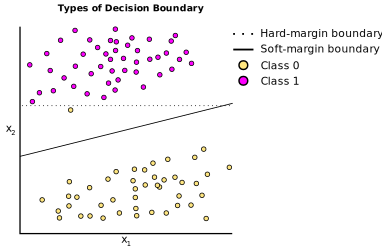
\includegraphics[width=\textwidth]{boundary.pdf}
    \caption{Demonstration of the utility of a soft-decision boundary to improve the overall
    fit of a decision boundary by allowing a degree of misclassification during training}
    \label{fig:boundary}
\end{figure}




\begin{figure}[h]
    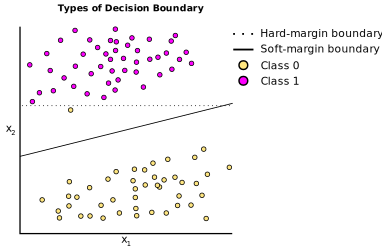
\includegraphics[width=\textwidth]{boundary.pdf}
    \caption{Demonstration of the utility of a soft-decision boundary to improve the overall
    fit of a decision boundary by allowing a degree of misclassification during training}
    \label{fig:boundary}
\end{figure}



SVMs are very good with low training datasets, and fast to classify (if not train) 







\subsection{Unsupervised Learning}

The other main form of machine learning is that of unsupervised or descriptive learning.
In which the training dataset has no provided output labels (y) i.e. 
\(\mathcal{D} = {x_{i} \forall i \in N}\) (where again N is the cardinality of 
this training dataset). In other words, we just have our dataset and have no additional information.
This is slightly more difficult problem as it lacks an obvious error metric like supervised learning 
(i.e. difference between actual output and expected output) but is important and useful tool to
try to discover patterns in datasets.

There are two major groups of unsupervised learning algorithms, the first of which is clustering algorithms
such as K-means that seeks to partition a dataset into a set of groups (see \ref{k-means} for more details).
The other major group of unsupervised algorithms are those used for visualisation and/or
dimensionality reduction.  Dimensionality reduction is a way of projecting a multidimensional
dataset into a lower number of dimensions in a way that still corresponds to
``shape'' of the data in the original number of dimensions.  

Formally, dimensionality reduction seeks to take a set of data (\(\mathcal{D}\)) and convert it
to a lower dimension form \(\mathcal{Y}\) known as a map \(\mathcal{Y} = {y_{i} \forall i \in N}\) 
with each individual \(x_{i}\) in \(\mathcal{D}\) represented by a corresponding map point \(y_{i}\). It
also seeks to do this in a way that maintains as much of the structure found in the original data 
as is possible \citep{Maaten2008} therefore, if two data points are similar in the original dimensions
they should still be similar in the map \(\mathcal{Y}\) (and the inverse).
Some dimensionality reduction approaches are well known in biology, specifically: principal component analysis (PCA) 
\citep{hotelling1933analysis} and multidimensional scaling (MDS) \citep{Torgerson1952} which both aim to identify
hidden features within the dataset that can explain a high degree of the variation.  


As ever different methodologies have a range of pros and cons, with
some better at preserving global structure (e.g. isomap) and others local data structures (e.g. local linear embedding) and so on.

One of the most recent innovations in this area is that of t-distributed stochastic neighbour-embedding
(t-SNE) in which the similarity of data points in the input space is modelled as pairwise probabilities 
using Gaussian distributions.
These probabilties are then translated into positions in the map \mathcal{Y} and similarities re-calculated
using Student's t-distributions.  The position and variance of these points and distributions respectively
is then optimised by mininising the difference between the similarity probabilities in the input space
and on the map \citep{Maaten2008}.

\subsubsection{K-means}

K-means clustering is a non-probabilistic unsupervised learning 
method in which we seek to partition data points in multidimensional space into 
K clusters. It is often used to initialise Gaussian mixture models.

Specifically, given a set of \(N\) observations \(X = {x_{1},...,x_{N}}\) 
of \(\mathcal{D}\) dimensions partition each point \((x_{n})\) into K clusters

A cluster can be intuitively considered as a group of observations/points which are 
``closer'' to one another than to other observations and the k-th cluster can 
defined by a \(\mathcal{D}\) dimensional vector \(\mu_{k}, where k=1,..,K\) for all clusters.
This vector represents the current ``prototype'' centroid of cluster. 

So, with k-means clustering we actually seek the set of K cluster centroids \({\mu_{k}}\) 
which minimise the sum of squares distances of each data point from its closest cluster centroid.
\citep{Bishop2006}

If we define a 1-of-K coding scheme with \(r_{nk} \belongs {0,1}\) as a binary variable that is 1 when \(x_{n}\) has been
assigned to cluster \(k\) (with centroid \(\mu_{k}\)) and 0 otherwise then we can define an objective cost function (\(J\)) 
that represents the sum of squares distances of each data point \(x_{n}\) from its assigned cluster centroid \(\mu_{k}\).

\[ 
    J = \sum_{n=1}^{N}\sum_{k=1}^{K} = r_{nk} \|x_{n} - \mu_{k}\|^{2}
    \label{eq:kmeans_cost}
\]

Therefore, the goal of k-means clustering is to find values for \({r_{nk}}\) and \({\mu_{k}}\) that minimise this linear 
function \ref{eq:kmeans_cost}.
\citep{Bishop2006}


The standard algorithm proceeds in two alternating steps following the initialisation of \(\mu_{k}\) with starting
cluster centroid locations \citep{Forgy1965,Lloyd1982}:
\begin{enumerate}
    \item \(\argmin_{r_{nk}} J\) i.e. minimise \ref{eq:kmeans_cost} w.r.t the assignment of points to clusters while keeping
        the cluster centroids fixed.
    \item \(\argmin_{\mu_{k}} J\) i.e. minimise \ref{eq:kmeans_cost} w.r.t the position of the cluster centroids while keeping
        the assignment of points to centroids fixed.
\end{enumerate}

Step 1 roughly corresponds to the expectation step in the expectation-maximisation (EM) algorithm and is trivially achieved by 
assigning each point to the cluster represented by the nearest centroid or formally:
\[
    r_{nk} = 
    \begin{cases}
        1,& \text{if} k=\argmin_{j} \|x_{n} - \mu_{j}\|^{2}\\
        0,& \text{otherwise}
    \end{cases}
\]

Step 2 roughtly corresponds to the maximisation step in EM is can be determined by taking the partial derivative of \(J\) w.r.t 
\(\mu_{k}\) setting it to 0 and solving for \(\mu_{k}\):
\[
    \frac{\partial J}{\partial \mu_{k}} = 2 \sum_{n=1}^{N} r_{nk} (x_{n} - \mu_{k})
    0 = 2 \sum_{n=1}^{N} r_{nk} (x_{n} - \mu_{k})
    \mu_{k} = \frac{\sum_{n} r_{nk}x_{n}}{\sum_{n} r_{nk}}
\]

In otherwords set \(\mu_{k}\) to the mean of all data points \(x_{n}\) assigned to cluster \(k\) thus k-means \citep{Bishop2006}

These two steps are repeated until a specified maximum number of iterations are reached or no points change cluster assignment during
step 1.

\(J\) \ref{eq:kmeans_cost} will converge but is liable to get stuck in a local rather than global minimum.

K-means has many modifications and improvements such as refinining the initialisation of the clusters by 
the Bradley-Fayyad method (clustering random samples of the dataset and then k-means clustering the resulting clusters) \citep{Bradley1998} 
or overclustering (running more than k-means clustering with more than the specified number of clusters and merging clusters at the end
to generate the correct number of clusters).

An efficient implementation of the k-means algorithm is available in the MLPACK C++ Machine Learning library \citep{mlpack2013}.






Disadvantages of K-means, requires a specified number of clusters (therefore diagnostics to check number of clusters)
Can converge to local optima.

Ways of specifying numbers of clusters \(k \equivalent \root{\frac{N}{2}}\) or information criteroin



\begin{figure}[h]
    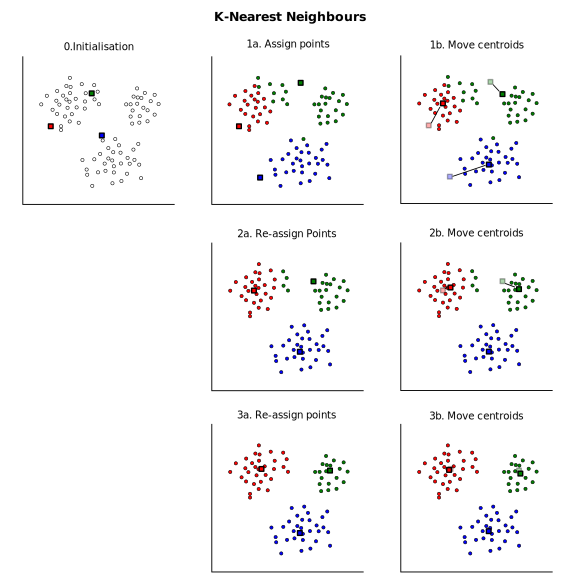
\includegraphics[width=\textwidth]{knn.pdf}
    \caption{Demonstration of the KNN algorithm applying 3 rounds of Expectation-Maximisation (labelled
    1a,2a,3a, and 1b,2b,3b respectively) }
    \label{fig:knn}
\end{figure}




%\subsubsection{t-Distributed Stochastic Neighbour Embedding (t-SNE)}
%t-SNE is recently developed unsupervised visualisation/dimensionality reduction algorithm 
%created by Hinton and van der Maaten \citep{Maaten2008}
%
%t-SNE converts the high-dimensional input data \mathcal{D} into a set of probabilities that represents
%how similar each pair of points are to one another.  Specifically, a student's t-distribution
%is centered on each data point with a specified variance  
%
%Specifically, \[
%    \text{similarity of point} \(x_{i}\) \text{to} \(x_{j}\) = p_{j|i}
%    p_{j|i} = \frac{\exp{\frac{-x ||x_{i} - x_{j} ||^{2}}{2\sigma^{2}_{i}}}}{
% 
%
%
%
%Data that forms distinct groups in t-SNE but overlap in PCA indicates datasets that are not
%linearly separable but may be amenable to non-linear methods.







\section{Phylogenetics}

Phylogenetics is an effective tool to investigate the evolutionary ancestry of biological sequence data.
It can be used to identify how closely related a given pair of sequences are, as
well as indicate what the sequence most likely looked like in a shared common
ancestor (ancestral node reconstruction). Phylogenetic methods also allow estimation
of evolutionary processes such as selection pressure,
migration, genome reduction, and horizontal gene transfer.
In the context of endosymbiosis, phylogenetics can be used to determine evolutionary ancestry of 
the genes recovered in a transcriptome and to aid identification the likely origin 
(host, endosymbiont, contaminant) of these transcripts. Additionally, it can pinpoint
likely horizontal gene transfer events between host and endosymbiont by searching for single 
gene/transcript phylogenies that have an incongruent branching pattern
compared to established species trees.  Finally, it can be used to aid identification of the likely function 
of novel transcripts based on similarity to other transcripts of known function in various
databases such as genbank.

Molecular phylogenetics brought a degree of statistical objectivity to philosophical principles of Willi Hennig's cladistics \citep{Felsenstein2001}


Phylogenetics can be defined as a means of arranging a set of character sequences into an optimal hierarchial
branching tree structure reflecting some measure of relatedness 
between the sequences (and occasionally other criteria). Usually, these trees will have variable
branch lengths that are product of a measure of divergence between the connected nodes.

Typically, these sequences take the form of protein or DNA sequences\footnote{
Strictly phylogenetics refers to the study of molecular sequence data although the same methods are applicable to
non-molecular characters such as morphological traits (and occasionally originated in this domain) as well as any
other set of discrete data vectors. It has even been applied to fields such as linguistics \citep{}
} and the measure of relatedness is some proxy for evolutionary distance ranging from simple distance measures 
e.g. Hamming distance (\(D = \sum_{k=0}^{N}|x_{k} - y_{k}|\) for two sequences \(x\) and \(y\) of length \(N\))
to more complicated probablistic estimations based on observed data.
A character is an element of a sequence such as an individual base or amino acid, homologous 
characters are those in separate sequences that are descended from a common ancestor.  
As they were the first molecular sequences easily available much of the early work in molecular phylogenetics
was conducted using protein sequences e.g. \citep{eck1966atlas,fitch1967}.

This phylogenetic estimation can be a non-trivial process (especially with more complex
measures of relatedness) as the number of
possible trees rapidly increases with the number of sequences \(N_{trees} = \prod_{x=2}^{N_{taxa}} (2x - 3)\).
However, the key stages in a phylogenetic analysis are that of sequence sampling,
 alignment (in which homologous sites in the sampled sequences are aligned with one another),
 masking (in which sites which are evolutionarily informative – can be determined to be homologous 
     but also non-invariant are selected), model selection (in which the best fitting
 evolutionary model is selected) and finally, phylogenetic reconstruction (in which the tree
 is generated that minimises some measure e.g. most likely tree for probabilistic models or 
 least distance).



One consideration worth raising is that increasingly it is becoming apparent
 that a tree-like pattern of evolutionary descent does not necessarily best represent
 actual evolutionary relationships.  This is due to the frequency of horizontal gene transfers (HGT)
 between distinct organisms (i.e. branches in a species trees).


Most analyses in this PhD are conducted using amino acid sequences.  
DNA is more likely to display a compositional bias, indepdence of sites
is often severely violated due to the structure of codons (3rd base wobble and so on)
(non-synoynmous mutations more likely to become fixed whereas synonymous mutations are
prone to drift).  Amino acids also have more states so are less susceptible to back mutations
than DNA.  





Supertree generate tree for each gene and use heuristic algorithm to combine \citep{Bininda-Emonds2004}, can spot HGT but is inefficient

Supermatrix, concatenation \citep{DeQueiroz2007a} - ignore differences in dynamics between gene, if partitioned then same as supertree



Best approach is supermatrix with a model that incoprotates rate heterogeneity \citep{Ren2009}



\subsection{Sequence sampling}
Sequence sampling, the selection and identification of sequences for initial inclusion in a 
phylogenetic analysis, is arguably the most important stage in phylogenetic analysis.
Any biases introduced here will propagate throughout the rest of the analysis. 
While some biases can be mitigated to lesser and greater extents 
by careful application of various methods in the following
stages, there is a degree of fundamental truth in the statement ``garbage in - garbage out''.




The aim of proper taxon sampling is to maximise phylogenetic accuracy and to allow
testing of specific hypotheses. 
Phylogenetic accuracy is usually considered in terms of consistency (as data increases 
    the analysis tends towards the correct tree), efficiency (how quickly does this convergence
occur), and robustness (how sensitive is the phylogeny to violation of assumptions in reconstruction) \citep{Nabhan2012}

The main issues caused by poor taxonomic sampling in molecular phylogenetics are that
of conflicting phylogenetic signals, inadequate rate of evolution to resolve relationships
of interest, and violations of assumptions e.g. expectation of a uniform distribution of traits \citep{Nabhan2012}.



Most contemporary models of phylogenetic inference only infer unrooted trees. 
Therefore, it is common practice to ``root a tree'' by selecting a set of sequences from known evolutionarily distance
organisms to form an outgroup. If this outgroup is correctly recovered (monophyletically) the root can be placed between
it and the other sequences in the phylogeny \citep{Yang2012}.  Additional, prior information is also occasionally used
to place restrictions on the tree topology such as known organismal relationships and fossil data.




Generally, increased taxon sampling has a strong positive effect on phylogenetic accuracy \citep{Zwickl2002}
however, it can also lead to a situation where there are too many sequences to efficiently
reconstruct a phylogeny.


and this 

However, care care must also be taken not to unintentionally bias datasets by removing 
any sequences that are considered ``problematic'' especially when conflicting phylogenetic signal
or model violations can be biologically informative.  Therefore, it is usually necessary to include
borderline error-generating sequences within a phylogeny initially and to iteratively remove them
and repeat the phylogenetic inference.


Compositional bias 


Long branch attraction is one of the most famous artefacts, it is the erroneous grouping of long (usually fast evolving)
branches in a tree as sister groups.  It is caused by 


Sequence sampling is important both between taxa and within taxa.

Hidden paralogy is another artefact that can be exacerbated with poor taxon sampling, this occurs when a sequence has
been duplicated within an ancestral taxa (creating paralogs) but differentially lost in its descendents.  
If, due to either deletion or poor sampling, the incorrect paralog is incoporated into a phylogeny 


Homoplasy - convergent evolution
Poor taxon sampling that is unrepresentative of the diversity that the phylogenetic tree
is intended to span 



With increasing size of available datasets a problem has emerged of acquiring too many homologous 
sequences to easily/feasibly use for phylogenetic inference.  Generally, this can and is typically reduced
to a representative subset by largely bias-prone heuristics or naive clustering.  However,
tools exist that utilise taxonomic database information to automatically a subset of specified
cardinality of sequences that display the maximium possible taxonomic diversity for that subset size \citep{Zhou2014}.


It is key to producing consistent, efficient and robust trees. 

Bias, long branches


The two principal ways in which putatively homologous sequences are identified in
sequence databases are those based upon Basic Local Alignment Search Tool (BLAST) and
its variants and Hidden-Markov Model based approaches (HMM).

\subsubsection{BLAST}

BLAST, its variants and improvements are the most widely used algorithms currently used to search sequence databases.
Fundamentally, they are sequence 

Likely homologous sequences can be identified via weak but biologically significant sequence similarities to a
given query sequence.



A variation BLAT (Basic Local Alignment Tool)




to identity likely homologous sequences 
to a given query.



\subsubsection{HMM}


\subsection{Multiple Sequence Alignment}

Arguably the most important step in phylogenetics is that of multiple sequence
alignment (MSA).  The goal of MSA is to align sets sequences such that 
evolutionarily homologous residues occupy the same column. In other words,
any given column in the alignment theoretically should contain amino acid or nucleotide residues
that derive from the same common ancestor and have evolved in each sequence lineage.
It is also possible that insertion or deletion events have taken place
and a particular residue is absent in the ancestral node or a sequence lineage.

This is a non-trivial computational problem which has been proven to have an NP-complete
\footnote{A decision problem for which an answer can be verified in polynomial time 
    by a non-deterministic turing machine and to and from which any NP-hard problem
    can be translated \citep{Karp1972}.} computational complexity \citep{Wang1994}.
Specifically, the optimal alignment of N sequences has a complexity of \[ O(L^{N}) \]
for \[ N\] sequences of length \[ L \]\citep{Sievers2011}.

Due to this complexity, the majority of MSA algorithms implement heuristic approaches
in order to get, if not the optimal solution, but a sufficiently good one in a reasonable
amount of time. 

Typically, MSA algorithms start by generating the sets of all pairwise alignments. 
This alignments are all generated 

Pairwise alignment algorithms are almost all based upon a
pair of ``Ur-algorithms'' with different goals: 
Needleman-Wunsch, a global alignment algorithms (which attempt to maximise 
alignment quality over entire sequence lengths) \citep{Needleman1970} and Smith-Waterman, 
a local alignment algorithms (which are optimised towards producing high quality alignments
in sub-strings) \citep{Smith1981}.  While early, MSA algorithms were typically
largely derived from Needleman-Wunsch most modern algorithms seek to combine 
optimisation of local and global alignments 


The mostly widely heuristic used to go from a series of pair-wise alignments to
a useful MSA is that of progressive-alignment \citep{Feng1987} (implemented in 
tools such as CLUSTAL W \citep{Thompson1994}) in which the pairwise alignment
scores are built into a distance matrix summarising the relative divergence of 
each pair of sequences. From this matrix a ``guide-tree'' is generated using simple
neighbour-joining methods (in which a tree is built by recursively clustering
the least dissimilar sequences \citep{Saitou1987}).  Sequences are then progressively
aligned using their branching order within this guide-tree \citep{Thompson1994}..
This drastically reduces the \[O(L^{N})\] complexity to approximately \[O(N^{2})\]
\citep{Sievers2011}. While there have been various improvements and alternative approaches
created such as merging both local and global alignment \citep{Notredame2000}, 
rapid identification of homologous regions using Fast Fourier Transforms \citep{Katoh2002},
iterative refinement of alignments \citep{Edgar2004a} and use of Hidden-Markov Models \citep{}<++>







That is the theoretical goal of MSA, however, clearly we cannot directly observe
the ancestral state of a residue in the common ancestor of two sequence lineages.
Therefore, MSA algorithms seek to indirectly infer a homologous alignment by 
introducing gaps into sequences in order maximise
an alignment ``score'' in which matches or alignments of more frequent
substituions (e.g. Leucine and its isomer Isoleucine or Adenine to its fellow purine base
Guanine (transition)) are positively scored and gaps (extension of a gap is typically
less penalised than creating a gap) or unlikely changes (e.g. the transversion
of Adenine to Cytosine or Glutamine to Cysteine) penalised.

This will generally be codified in a substitution matrix e.g. the PAM \citep{Dayhoff1978}, 
BLOSUM \citep{Henikoff1992} amino acid matrices and their numerous subsequent
derivations and improvements. 




Using these matrices MSA algorithms will typically
align pairs of sequences and then use this set of pairwise-alignment scores
to estimate a ``guide tree''.  This guide-tree is then used to infer the order 
in which the MSA is built








There have been compelling arguments as early as 1991 that MSA are inherently flawed as consideration of 
evolutionary processess in the objective weighting and assessment of potential alignments \citep{Thorne1991}.
Furthermore, joint inference of alignment and phylogenetic trees minimises the risk
of conscious or subconscious research bias towards alignments and subsequent 
phylogenies that support their pre-conceived ideas.


and trees should be jointly inferred \citep{Thorne1991,Bouchard-Cote2013}

bias that alignment and inferences should be jointly estimated \citep{Redelings2005}.
While, this approach has been coded in interest probabilistic programming approaches
such as that implemented in BALI-phy \citep{Suchard2006} it is still far too
slow a process to infer phylogenies in this manner on large or even moderate datasets.
Therefore, for now independent alignment estimation is here to stay, at least until
computation resources and algorithmic development has continued until these more
theoretically satisfying approaches become feasible.


\begin{figure}
    \caption{Redrawn from a slide by Derrick Zwickl
\end{figure}

\subsection{Masking}

Concatenation - assumes common evolutionary patterns


MSA is imperfect - especially for faster algorithms necessary with larger datasets
and higher throughput.

Trimming ambiguously aligned and absent sites improves phylogenetic accuracy \citep{Talavera2007}

Automating this process - score each column indepdendently  gap score, similarity score and/or consistency score
fraction of seq without gap, ss mean distatnce between residues, sc can be calced with multiple alignments of same seqs:
how consistently is a column found in different alignments 

Trimal automatically trims based on these thresholds \citep{Capella-Gutierrez2009}

\subsection{Substitution model selection}


Parsimony does not need a model.




Substitution models typically assume neutrality, independence and finite sites.
With the probability of substitution rates having an idendently identical distribution (i.i.d) \citep{Hasegawa1985}




Branch length is the expected number of substitutions per site.

This measure of distance can be naive models where rates of change between character
states and the frequency of each state is equal (e.g. \(p(x \rightarrow y) \forall x \forall y \in {G,C,T,A} \text{where} x\neq y\)
\citep{jukes1969evolution}) to models fully paramaterised in terms of character frequency and rates of change by the masked alignment 
(e.g. the generalised time-reversible (GTR) model \citep{Tavare1986} see \ref{eq:gtr})

\begin{figure}
    \[Q=\begin{pmatrix}
        . & \alpha\pi_{C}  & \beta\pi_{A} & \gamma\pi_{G}\\ 
        \alpha\pi_{T} & . & \delta\pi_{A} & \epsilon\pi_{G}\\ 
        \beta\pi_{T} & \delta\pi_{C} & . & \zeta\pi_{G}\\ 
        \gamma\pi_{T} & \epsilon\pi_{C} & \zeta_\pi_{A} & .
    \end{pmatrix}\\
    Q_{ii} = -\sum_{{j | j \neq i}} Q_{ij}\\
    \Pi = (\pi_{G}, \pi_{T}, \pi_{C}, \pi_{A})\\
    \Pi * Q = 0 \\
    \alpha = p(T \leftrightarrow C)\\
    \beta = p(A \leftrightarrow T)\\
    \gamma = p(G \leftrightarrow T)\\
    \delta = p(C \leftrightarrow A)\\
    \epsilon = p(G \leftrightarrow C)\\
        \zeta = p(A \leftrightarrow G)\]
        \caption{Generalised time-reversible model for DNA sequence evolution under a reversible homogeneous markov process where \(\Pi\) is the 
        frequency of each state and \(\alpha\) through \(\zeta\) are substitution rates \citep{Tavare1986,Yang1994}.  All other markov process models
    of sequence evolution are special cases of GTR.   Time-reversability refers to the fact that \(\pi_{i}Q_{ij} = \pi_{j}Q_{ji}\) therefore
   the direction of state changes is irrelevant}
        \label{eq:gtr}
\end{figure}

While models like GTR can feasibly be paramaterised 

In order to allow the oft violated assumption of a simple substitution that the rate of substitutions is constant (partially relaxes i.i.d)
across the alignment there are many improvements.  The most frequent of which allowing the rates to vary across
sites in the form of \(\Gamma\) distribution \(Var = \frac{\alpha}{\beta^{2}}, \mu = \frac{\alpha}{\beta}\) with a given shape \(\alpha\) and 
trivial scale factor \(\beta\) depending on the dataset 

For datasets that have a high degree
of rate heterogeneity a low valued \(\alpha\) produces a broad distribution of rates, whereas a high value will generate 
a narrow distribution for datasets with low rate heterogeneity \citep{Yang1993}.
For reasons of computational efficiency \(\Gamma\) is typically approximated as a discrete distribution of 4 to 8 
categories of equal probability \citep{Yang1994a}. 

A more limited version of this is the invariant sites model in which sites are divided into 2 classes, one considered invariable while the 
other has normal substitution rates applied \citep{Hasegawa1985}.

Unfortunately, these models still assume other model parameters namely the equilibrium frequencies and relative rates are the same across
sites.  Some models have been proposed with multiple rate matrices  \citep{Lartillot2004}



State frequency can be defined at each site \citep{Bruno1996} but needs lots of taxa \citep{Lartillot2004}
Mixture model with K classes each containing a different state frequency. if K=N sites then same as Bruno
if k=1 same as naive model.  DPP can be used to determine total number of classes \citep{Lartillot2004}


Can explicitly partition or use DPP etc and complex models - depends on prefrence for fixed-effects models or random-effects
\citep{Yang2012}


Codon models


Covarion model - heterotachy  variation of rate at a site across time  - site change between on and off (prop at each site is different)
covarion model using infinite mixture model\citep{Zhou2010} 








A model is stationary if Q does not change with time.


Regardless of how many sequences and how many characters are used to generate a phylogeny 

model selection is 
Maximum likelihood model

Simple models such as parsimony and distance approaches are more susceptible to artefacts such as LBA.



Distance, ML and Bayesian inferences also suffer from LBA if the assumed model does not account for rate variation using \Gamma etc \citep{Yang1996}



Advantage of model-based approaches is that assumptions are explicit and thus can be tested in a statistically robust manner.








actually choosing a model - prottest AIC/BIC/DT criteria - guide tree - matrix selection \citep{Abascal2005}
Review of model selection \citep{Sullivan2005}



\subsection{Phylogenetic inference}


The simplest phylogenetic inferences are that of distance matrix methods.
Distance matrix methods \citep{Fitch1967} work on the basis of generating 
a matrix representing the pairwise distances of each sequence using the selected
substitution model and inferring a phylogeny from this.  The simplest case
would be searching tree space for the optimal tree using a standard least-squares
criteria between actual and expected branch lengths (i.e. distances) \citep{Fitch1967,Cavalli-Sforza1967}.

However, the most common is that of neighbour-joining which begins with the distance matrix and a 
star topology tree in which all leaf node branches are connected to a single shared central node.
Then:
\begin{enumerate}
    \item Find the closest two branches in the distance matrix 
    \item Join the closest pair into a single branch with a new internal node connected to central node
    \item Generate a new distance matrix reducing the selected pair to the new node (     
        the distance of the selected pair of leafs to the new internal node 
    and the distance between every other leaf and the new internal node)
    \item Repeat the process with the new matrix \citep{Nei1987}
\end{enumerate}

It works on the assumption that the true tree has the smallest expected length (minimum evolution) and a short tree
that has similar topology can be achieved using the fast simple agglomerative algorithm.


NJ is one of the best distance methods and is more reliable than maximum-parsimony which can be asymptotically inconsistent

While already efficient (possibly efficient as possible) can be made more efficient using effective heuristics
to search tree space \citep{Kumar1996}

As well as improvements where variance is minimised instead of pure distance improving performance in datasets with high
substitution rates e.g. BIONJ \citep{Gascuel1997}



Distance methods are fast as they don't have to compare as many trees as MP or ML meothds \citep{} but can perform
very poorly for divergent sequences with large sampling errors as they don't generally account for variance in 
distance estimates \citep{Yang2012} (BIONJ kind of does).
They are also sensisitve to gaps in the alignment.





Parsimony approaches \citep{Camin1965} on molecular sequences \citep{eck1966atlas} seek to infer the maximum parsimony (MP) tree.
That is the tree which requires the smallest number of character changes (has the best tree score).  Where the tree score is the sum of 
all character lengths (the minimum number of changes for each site in the alignment).  Any site that is invariable is not
informative for generation of a parsimony tree.
It has no explicit assumptions relative to other methods however, this means it is difficult to build in 
prior knowledge of sequence evolution when generating a tree.

It also fails when multiple substitutions have occurred at the same site or with parallel changes in two long branches 
and therefore is especially prone to long-branch attraction.
\citep{Felsenstein1978}
Prestige of parsimony methods declined with discoveries that they can produce statistically inconsistent
phylogenies \citep{Felsenstein2001}






Bootstraps resampling data with replacement and reanalyse - variation estimates the aize of error in estimates \citep{Felsenstein1985}
Majority-rul conensus strees show number of trees supporting 





\subsubsection{Maximum likelihood}

Maximum likelihood methods seek to discover the maximum-likelihood estimates (MLEs) of the tree parameters (topology, branch length and usually substitution model parameters)
for the data.
These MLEs are estimated numerically using standard iterative optimisation algorithms.
%%%MLEs have been proven to be asymptotically have high phylogenetic accuracy (unbiased, consistent and efficient). for true tree not ML tree
MLE are proven consistent \citep{Wald1949} but the due to the complexity of phylogenetic inference
this proof does not apply \citep{Yang2012}

Explicit model assumptions,  can make use of sophisticated evolutionary models, 
almost all major published phylogenies use ML or bayes

LRTs can examine fit for evolutionary models: \(2ln(\frac{L_{1}}{L_{0}})\) \citep{Goldman1987}

ML is relative slow to calculate 


Likelihood models using symmetric changes between all proteins \citep{neyman1971molecular}
and more efficient implementations \citep{Felsenstein1981}

higher efficiency than distance or parsimony 

\subsubsection{Bayesian}

Bayesian inference is, as the name suggests, based on the Baye's therem.

\(p(\theta | D) = \frac{p(\theta)p(D|\theta)}{p(D)}\)

with \(p(\theta)\) being the prior probability for model parameters (topology, branch length, substituion model)
\(p(D|\theta)\) being the likelihood of the data given a certain set of parameters with \(p(D)\) as the marginal 
probability.

Due to the computational infeasability of directly calculating the marginal likelihood (integrated over all possible
paramater values in all dimensions) phylogenetic inference uses MCMC 


Posterior probabilityes so no need to calculate bootstraps 

PP sensitive to model violations
Prior lets new data added  but difficult to specify with complex pathologies 
Bayesian robutness analysis is important when setting priors 

Chain length is highly data dependent

slower


Robuse to missing data \citep{Wiens2008} so is ML







\section{Informatics languages and hardware}

\subsection{Languages and Libraries} 
Several programming languages and a range of libraries were used throughout this PhD depending
on the suitability of a particular tool for a task.
The full details of the specific tools used for the main analyses are outlined during the description
of these analyses, however, the tools used for prototyping as well as those used for smaller tasks not covered
in detail are omitted elsewhere. 

Languages and libraries were chosen depending on their best fit for a particular task.
Performance sensitive code such as those dealing with large datasets (e.g. high-throughput sequencing 
libraries or image data) were principally conducted using the C++ language 
in line with the C++11 standard \citep{ISOInternationalStandard2011}

The main C++ libraries used in addition to the C++11 standard library were:
\begin{itemize}
    \item Seqtk - fastq/a sequence parsing library \citep{SeqtkGitHub}
    \item MLPACK - a high-performance machine learning library \url{http://www.mlpack.org/} \citep{mlpack2013}
    \item OpenCV3 - widely used computer vision library \citep{opencv_library}
    \item Armadillo - numerical computation library \citep{Sanderson2010}
\end{itemize}

The majority of tasks were accomplished using the high-level python language (python2.7 or python3.4
depending on the application) \citep{}.  In addition to the standard library, the numerical
computation libraries numpy \citep{} and theano \citep{}, machine learning library scikit-learn \citep{},
statistical and scientific libraries scipy \citep{} and pandas \citep{}, the bioinformatics libraries
scikit-bio \citep{} and biopython \citep{}, and plotting libraries holoviews \citep{}, 
matplotlib \citep{} and bokeh \citep{} were all used extensively.
Frequent use was made of literate programming offered by environments such as the ipython notebook (recently
renamed jupyter).

The statistical programming language R \citep{RCoreTeam2015} was used for some data analysis
and visualisation primarily using ggplot2 \citep{Wickham2009} and dplyr \citep{Wickham2014}.
This was primarily done using the R-Studio \url{http://www.rstudio.com/} integrated development environment) and 
R-markdown \citep{Allaire2014}.

All code was version controlled using git \url{http://git-scm.com/} and remotely hosted using github \url{https://github.com/} and bitbucket \url{https://bitbucket.org/} 
services.  Unit tests were automatically run on synchronisation (`push') with these remote servers using 
the Travis \url{https://travis-ci.org/} Continuous Integration service.

Incidental scripting was done using zsh and bash languages and all code was written using a simple vim terminal.

\subsection{Hardware}

All analyses were conducted on either the lab cluster (running Ubuntu Server LTS 12.04 and 14.04 \url{http://www.ubuntu.com}:
\begin{itemize} 
    \item PowerEdgeM910 with 2 x Intel Xeon CPU \(E6510 @ 1.73GHz, 512GB\) RAM
    \item PowerEdgeM910 with 2 x Intel Xeon CPU \(E7-4807 @ 1.87GHz, 512GB\) RAM
    \item PowerEdgeM620 with 2 x Intel Xeon CPU \(E5-2650 v2 @ 2.60GHz, 512GB\) RAM
\end{itemize}
Or on two workstations both running continuously updated versions of Arch Linux \url{https://www.archlinux.org/}.
\begin{itemize}
    \item Apple MacPro with 2 x Intel Xeon CPU \(E5520 @ 2.27GHz, 16GB\) RAM
    \item Dell Precision T7500 with 2 x Intel Xeon \(E5620 @ 2.4GHz, 48GB\) RAM
\end{itemize}

\section{OLD CRAP}
%\subsection{RNA-Seq}
%Transcriptomics and specifically RNA-Seq is one of the key investigative techniques that will be used in this project.  
%By extracting and sequencing mRNA expressed by host and endosymbiont during day and night conditions we will identify key genes involved in endosymbiotic interactions.
%RNA-seq is a second-generation sequencing technology developed to perform high-throughput short-read sequencing of cDNA generated from extracted RNA [Grabherr, 2011]. 
%As ribosomal RNA forms such a significant portion of cellular RNA it is necessary to remove it before sequencing in order to make meaningful inferences of transcript expression.  
%This can be achieved either by ribosomal depletion in which ribosomal sequences are bound by adaptors which in turn bind to magnetic beads allowing the mechanical removal of these molecules.  
%This methodology allows the preservation of smaller non-coding RNAs present in the system. However, as we are principally interested in transcripts and are operating in a eukaryotic system with poly-adenylated mRNA we can efficiently isolate mRNA via a poly-A selection, in which poly-T primers are used in reverse-transcription of mRNA into cDNA.
%From this point RNA-Seq proceeds in the same manner as other next-generation sequencing methods. 
%We are using a method known as paired-end sequencing (available on the Illumina HiSeq 2000 platform) in which 76bp reads are sequenced at either end of a 200-500bp insert. 
%This improves the ease of transcriptome assembly by providing additional positional information when producing de-Bruijn graphs. 
%
%\subsection{Transcriptome Assembly}
%Assembly is the process by which the short high-throughput sequencing reads are combined to recover the longer transcripts from which they have been randomly sampled.  
%In the simplest sense, this process relies on the quality score weighted alignment of reads.  
%Transcriptome assembly can be done in two ways: referenced (in which reads are aligned to a reference genome), and de-novo (in which the reads are assembled without a reference).  
%De-novo assembly are mainly conducted using k-mer based de-Bruijn graph creation.  
%Very briefly, reads are subdivided into k-mers (\textasciitilde $15-30$ nucleotide sequences) to aid in computation and then assembled in graphs based on k-1 overlaps between k-mers.
%With the exception of repeated regions the transcript is recovered by finding the shortest path around the graph visiting all vertexes once (i.e. a hamiltonian path). 
%In reality, assembly algorithms weight the construction of these k-mers and graphs using sequence quality scores and a large number of established heuristics.
%Referenced assemblies are often considered sub-optimal in some eukaryotic organisms due to alternative splicing and other transcript modifications not directly represented in the genomic sequences.  
%Despite this, for a \textit{Paramecium - Chlorella} transcriptome, host transcripts could still potentially be assembled as the closest available genome sequence is that of the \textit{Paramecium tetraurelia} macronuclei in which most intronic elements have been spliced out [Mayer \& Forney 1999].  
%However, using this genome as a reference for the assembly of host transcripts may be highly misleading due to the fact that this organism does not harbour \textit{Chlorella} endosymbionts and thus may lack the genes required to maintain this system and also has undergone two rounds of whole genome duplication since sharing a common ancestor with \textit{Paramecium bursaria} potentially leading to high levels of sequence divergence.  
%On the other hand, endosymbiont transcripts could be assembled using the endosymbiotic \textit{Chlorella} NC64A genome [Blanc et al., 2010] once the relationship between this organism and the endosymbiont within the CCAP 1660/12 culture is determined phylogenetically and is determined as meaningfully close.  However, the potential issue of alternative splicing would occur if we were to use this genome sequence.  
%Therefore, our initial assembly was conducted de-novo (i.e. without any reference genomes) in order to attempt to avoid biasing due to these reference genomes.   
%
%
%\subsection{Phylogenetics}
%The next key method in this project is that of phylogenetics as it is an effective tool with which to investigate the evolutionary ancestry of the genes recovered in the transcriptome and to identify the likely origin (host, endosymbiont, contaminant) of these transcripts.  
%It can also be used to identify potential horizontal gene transfer events between host and endosymbiont by searching for single gene/transcript phylogenies that have an incongruent branching pattern compared to established species trees.    
%
%\subsection{Annotation}
%In order to identify proteins putatively involved in endosymbiosis – namely transporters and secreted proteins and to identify proteins likely involved in their regulation it is necessary to functionally annotate assembled transcripts.  
%This was achieved in a variety of ways including Hidden-Markov Models or HMMs (via HMMer, PFAM and other similar resources), alignment (via BLAST), KEGG Ontology and Gene Ontology annotation (via tools such as the KEGG Automated Annotation Server or BLAST2Go). 
%HMMs are a commonly used tool in sequence identification and depending on their training are generally more sensitive than alignment based methods [Eddy., 2011].
%This will be further discussed within the methods.
%
%\section{Methods}
%\subsection{Culturing}
%
%\subsection{RNA-Seq}
%\subsubsection{cDNA generation and library preparation}
%
%Purified RNA from day and night samples were pooled into a single day and a single night sample due to limitations on the quantity of extracted RNA. 
%These two samples were then prepared for sequencing using the TruSeq Stranded RNA preparation kit (Illumina).  
%mRNA was selected using a poly-A selection method before being fragmented, cleaned-up using ethanol and then reverse transcribed into single-stranded cDNA using random hexamer primers. 
%The prepared ds cDNA was then end-repaired or cleaved to produce blunt-ended fragments.  
%By the addition of a trailing A-base to these fragments sequencing adaptors were added using an overlapping complementary T-base.  
%Fragments were then denatured and amplified before cluster generation using the standard Illumina sequence library preparation methods [\url{http://res.illumina.com/documents/products/datasheets/datasheet_truseq_sample_prep_kits.pdf}].
%
%\subsubsection{Sequencing}
%
%Clonal cluster generation by bridge amplification was conducted on the cBot (Illumina) platform using the TruSeq Paired-End cluster kit (Illumina).  
%The samples were run in individual lanes on a HiSeq 2000 8-lane flow-cell (Illumina) to produce 76bp paired-end reads. 
%Sequencing was conducted at the University of Exeter sequencing service.
%
%\subsubsection{Assembly}
%The paired-end fastq reads from the sequencing experiment were trimmed to sequences of sufficient quality and sequencing adaptors removed. 
%Reads from day-and-night runs were assembled separately as well as a combined assembly of all the reads. 
%As the \textit{Paramecium bursaria} 1660 genome or the \textit{Chlorella} endosymbiont (CCAP12) have not yet been sequenced de-novo transcriptome assembly was conducted (further explanation for this in background section).  
%This was done using both the Oases package [Schluz, 2012] from European Bioinformatics Institute [\url{http://www.ebi.ac.uk/~zerbino/oases/}] and the Trinity package [Haas, 2013] provided by the Broad Institute [\url{http://trinityrnaseq.sourceforge.net/}] using a high-memory computing cluster at the University of Exeter.  
%Assemblies were compared and a single assembly methodology was selected for further downstream analysis. 
%
%\subsubsection{Saturation}
%In order to assess whether increased sequencing depth would recover further transcripts a read-saturation analysis was conducted.  
%This was achieved by developing a program to repeatedly take random subsamples of the paired-end reads (from the day sample, the night sample and the combined pool) and assessing the number of the assembled transcripts that could be successfully recovered using these reads.  
%This was done with the aid of a short-read aligner bowtie-2 [Langmead, 2012], standard GNU/Linux command line tools, and a custom python script.  
%The results were plotted using python+matplotlib and assessed for saturation in transcript recovery
%
%\subsubsection{Extracting Likely Coding Regions}
%As host and endosymbiont use different codon tables it was necessary to identify ORFs in the assembled transcripts using both tetrahymena (i.e. Host/Paramecium) and universal (endosymbiont/Chlorella and bacterial contaminant/foodstock) encodings.  
%The ciliate `tetrahymena' encoding differs from universal codon look up tables in that UAA and UAG which are normally stop codons instead code for glutamine, this means \textit{Paramecium} only has a single stop codon (UGA) [Harper \& Jahn, 1989].
%This was conducted using the Trinity transcripts\_to\_best\_scoring\_ORFs tool [\url{http://trinityrnaseq.sourceforge.net/analysis/extract_proteins_from_trinity_transcripts.html}].  
%Initially, this tool identifies the longest ORF within each assembled transcript.  
%These longest ORFs are used to train a hexamer-based HMM which is then used to identify the ORFs with highest likelihood.  
%These ORFs are then translated into peptide sequences. 
%
%\subsubsection{Transcript Identification}
%Despite care being taken in filtering and washing-off bacteria from the \textit{Paramecium} prey food-stock and usage of poly-A selection, bacterial contamination was still present in our assembled contigs.  
%Therefore, it was necessary to develop a pipeline to identify the transcript origins to filter those transcripts originating from host and endosymbiont. 
%Initially transcripts were binned into their predicted source - Host (H), Unknown but likely Host (U(H)), Endosymbiont (E), Unknown but likely Endosymbiont (U(E)), Food (F), Unknown but likely Food (U(F)), and Unknown (U).  
%Each of the assembled transcripts were BLASTed against a database consisting of the following genomes: \textit{Chlorella} NC64A, \textit{Chlamydomonas reinhardtii}, \textit{Coccomyxa} C169, \textit{Paramecium tetraurelia}, \textit{Tetrahymena thermophila},  \textit{Arabidopsis thaliana}, \textit{Homo sapiens} (helping to identify contamination), \textit{Saccharomyces cerevisiae}, \textit{Schizosaccharomyces pombe}, \textit{Bacillus cereus} ATCC 14579, \textit{Escherichia coli} 536, \textit{Escherichia coli} O157 H-7, \textit{Salmonella typhimurium} LT2 and \textit{Escherichia coli} K-12 (the last 5 genome datasets helping to identify food bacterial genes).  
%The bins were classified as follows:
%\begin{itemize}
%  \item Endosymbiont (E): Transcript's highest scoring BLAST hit at -50E was to \textit{Coccomyxa}, \textit{Chlamydomonas} or \textit{Chlorella}.  Or transcript's highest scoring hit at -20E was one of those species and the longest likely coding region in the transcript was using the universal codon table. 
%  \item Unknown but likely Endosymbiont (U(E)): -10E hit to \textit{Coccomyxa}, \textit{Chlamydomonas} or \textit{Chlorella} and longest likely coding region was using the universal codon table. Or transcript's highest hits at -10E and -20E were to one of those genomes regardless of coding region presence.
%  \item Host (H): Transcript's highest hits at -50E were to \textit{Paramecium tetraurelia} or \textit{Tetrahymena thermophila}.  Or highest hit at -20E was one of those species and longest likely coding region was using the Tetrahymena codon table.
%  \item Unknown but likely Host (U(H)): -10E hit to \textit{Paramecium tetraurelia} or \textit{Tetrahymena thermophila} and longest likely coding region was was using the Tetrahymena codon table. Or transcript's highest hits at -10E and -20E were to one of those genomes regardless of coding region presence.
%  \item Food (F): Transcript's highest scoring BLAST hit at -50E was to one of the \textit{E. coli} species or \textit{Salmonella}.  Or transcript's highest scoring hit at -20E was one of those species and the longest likely coding region in the transcript was using the universal codon table.
%  \item Unknown but likely Food (U(F)): -10E hit to one of the \textit{E. coli} species or \textit{Salmonella} and longest likely coding region was using the universal codon table. Or transcript's highest hits at -10E and -20E were to one of those genomes regardless of coding region presence.
%  \item Unknown (U): highest scoring hits to \textit{Arabidopsis}, \textit{Homo sapiens}, \textit{Saccharomyces} or \textit{Schizosaccharomyces} or any sequence not fitting into the above categories.
%\end{itemize}
%
%In order to assess the accuracy of the `binning' of endosymbiont sequences and to estimate how many host or endosymbiont transcripts we would accidentally discard using these categories we used a phylogenetic analysis pipeline to verify the likely ancestry and therefore point of origin within the endosymbiosis of each sequence.  
%A script was created used the translated transcript peptide sequences to search a database of over 900 representative genomes using BLASTp.  This script recovered all sequences above an E-value of $10^{-5}$. 
%These sequences were then automatically aligned and masked using MUSCLE [Edgar, 2004] and TrimAL [Capella-Gutierrez, 2009]. 
%Fast maximum-likelihood trees were then generated for each masked alignment using FASTREE2 program [Price, 2010].  
%These trees were then converted to scalable vector graphics and using the NCBI taxonomy API each branch was colour coded depending on taxonomic group.  
%This allowed for quick manual inspection to determine the likely origin identity of the initial transcript.  
%For example, if a transcript sequence was found to branch largely within archaeplastida species it was considered as likely originating from the endosymbiont.  
%Likewise, if it branched largely among ciliate species it was considered as likely host-derived.  
%Continuing in the same vein, those sequences considered as being derived from bacterial food-stocks were considered as those that branched largely within bacterial clades and those sequences that branched with no clear pattern were considered to be `Unknown'.  
%Any transcripts where endosymbiont sequences were found to branch incongruently with accepted topologies (especially within the ciliate or bacteria) were determined to be showing signs of potential horizontal gene transfers and were recorded for further analysis.  
%For example, if a transcript branched with another endosymbiotic algae (particularly \textit{Chlorella} NC64A) within a clade of ciliates this would be considered a potential HGT event to be further investigated.
%The entire initial `Endosymbiont Bin' (2,825 transcripts), the `Unknown but likely Endosymbiont Bin' (600) and the `Unknown Bin' (2,096) were phylogenetically tested using this pipeline.  
%However, owing to the size of the initial `Food Bin' (5,129) and `Host Bin' (27,907) it wasn't possible to exhaustively test all transcripts in these two bins therefore 2000 transcripts were randomly selected from each them and tested using the pipeline. 
%In the cases where too few sequences were recovered to produce a phylogeny (<3 including seed) the source proteomes of the sequences that were recovered were assessed. For example, if the recovered sequences were from the archaeplastida that was considered sufficient evidence to class that transcript as belonging to that `Endosymbiont Bin' and so on.  If no other sequences were recovered using BLASTp then the transcript was placed into the `Unknown Bin'.
%The change in initial binning after phylogenetic verification were then plotted using python+matplotlib and an estimate for the numbers of unidentified endosymbiont transcripts was made.
%
%\subsubsection{Identification of putative secreted and putative transporter proteins}
%Initial transcript functional annotation was conducted via BLAST and mapping Gene Ontology terms using the Blast2GO application [Conesa, A. et al., 2005] [\url{http://www.blast2go.com/b2ghome}].  
%In order to more accurately identify the likely proteins involved in the maintenance of the \textit{Paramecium-Chlorella} photosynthetic endosymbiosis we attempted to identify all transporter and secreted proteins within the verified endosymbiont and host transcript complements. A permissive set and conservative subset of host and endosymbiont transporter and secreted proteins were identified using a combination of pipelines.
% Putative transporter proteins were identified as all coding sequences within each bin containing 1 or more transmembrane domains (as identified by the HMM implemented in the program tmhmm 2.0c  [Krogh et al., 2001, Sonnhammer et al., 1998]).  
%The conservative subset of transporter proteins were those identified as containing 4 or more TM domains.  
%The predicted host and endosymbiont secretome was determined by combining the outputs of several established and widely-published programs for identification of secreted proteins - SignalP 4.1 [Petersen et al., 2011], tmhmm 2.0c, TargetP 1.1 [Emanuelsson et al., 2000], and WoLFPSORT 0.2 [Horton et al., 2007] (with the assistance of some accessory scripts from from UCSC [\url{http://hgdownload.cse.ucsc.edu/admin/exe/}] and the FASTX-toolkit [\url{http://hannonlab.cshl.edu/fastx_toolkit/index.html}]). 
%Input sequences were checked for the presence of N-terminal signal peptides primarily via the detection of signal peptide cleavage sites by the HMM implemented in SignalP 4.1. 
%Mature peptides (i.e. those with the detected signal peptide cleaved) output from SignalP 4.1 were then processed in tmhmm 2.0c to detect and remove any sequences containing transmembrane domains. 
%The output from these two stages were then combined with all initial input sequences detected as secreted (S) by TargetP 1.1 and as having an extracellular localisation via WoLFPSORT 0.2 to produce a single fasta formatted output file containing the entire predicted secretome, i.e. a set of proteins predicted to be secreted by all three bioinformatic methods. 
%This therefore identified the conservative subset of host and endosymbiont secreted proteins. 
%A second list of putative secreted proteins was identified as any protein predicted to be secreted by any one of either SignalP 4.1, WoLFPSORT 0.2, or TargetP 1.1. It must be noted that such prediction approaches are only as good as the quality of each individual transcript assembly. 
%Genes with low transcript levels are likely to have low coverage and assembly quality potentially leading to false negative detection of N-terminal signal peptides. 
%This was investigated in more detail below.
%
%\subsubsection{Coverage}
%As the identification of the secreted proteins hinged upon the recovery and accurate prediction of N-terminal signal peptides it was necessary to assess the position-specific read coverage across the transcript specifically at the C- and N- termini. 
%This was achieved by developing a script to count and average (median) the number of reads aligning to each nucleotide in both tetrahymena and universal (i.e. host and endosymbiont) likely coding regions using a custom python script.  
%This was done for all tetrahymena and universal coding regions in transcripts, all phylogenetically confirmed host and endosymbiont binned sequences, conservatively and permissively identified putative secreted and transporter proteins in the `Host Bin' and `Endosymbiont Bin'. 
%Results were then plotted using python+matplotlib.
%

